Другой метод предложенный авторами работы \cite{piezo50} заключается в измерении интенсивности для разной
отстройки от точного бреговского угла кристалла образца в двухкристальной схеме дифрактометра.
Необходимо  встать в произвольную точку на кривой дифракционного отражения,
другими словами выведем интенсивность детектора из максимума отражения в точку на склоне
 кривой (Рис.~\ref{ris:kdopiez}).

\begin{figure}[H]
\centering
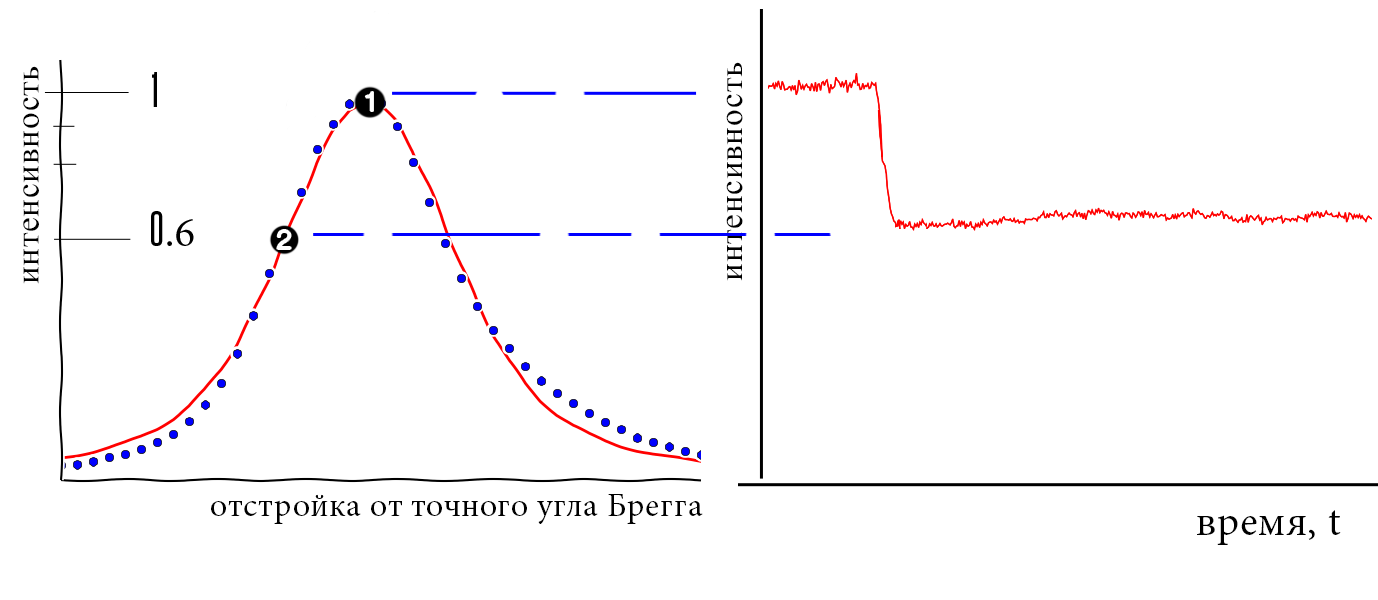
\includegraphics[width=1\linewidth]{images/kdopiez.eps}
\caption{Выбор точки на КДО(справа), интенсивность сигнала детектора(слева)}
\label{ris:kdopiez}
\end{figure}

При включении электрического поля (рисунок \ref{ris:princip}В) для разных направлений наблюдаем изменение интенсивности
на детекторе (рисунок \ref{ris:princip}А). Изменение интенсивности характеризует динамику смещения
двухкристальной КДО (рисунок \ref{ris:princip}C) из-за изменения межплоскостного расстояния в образце.

\begin{figure}[H]
\centering
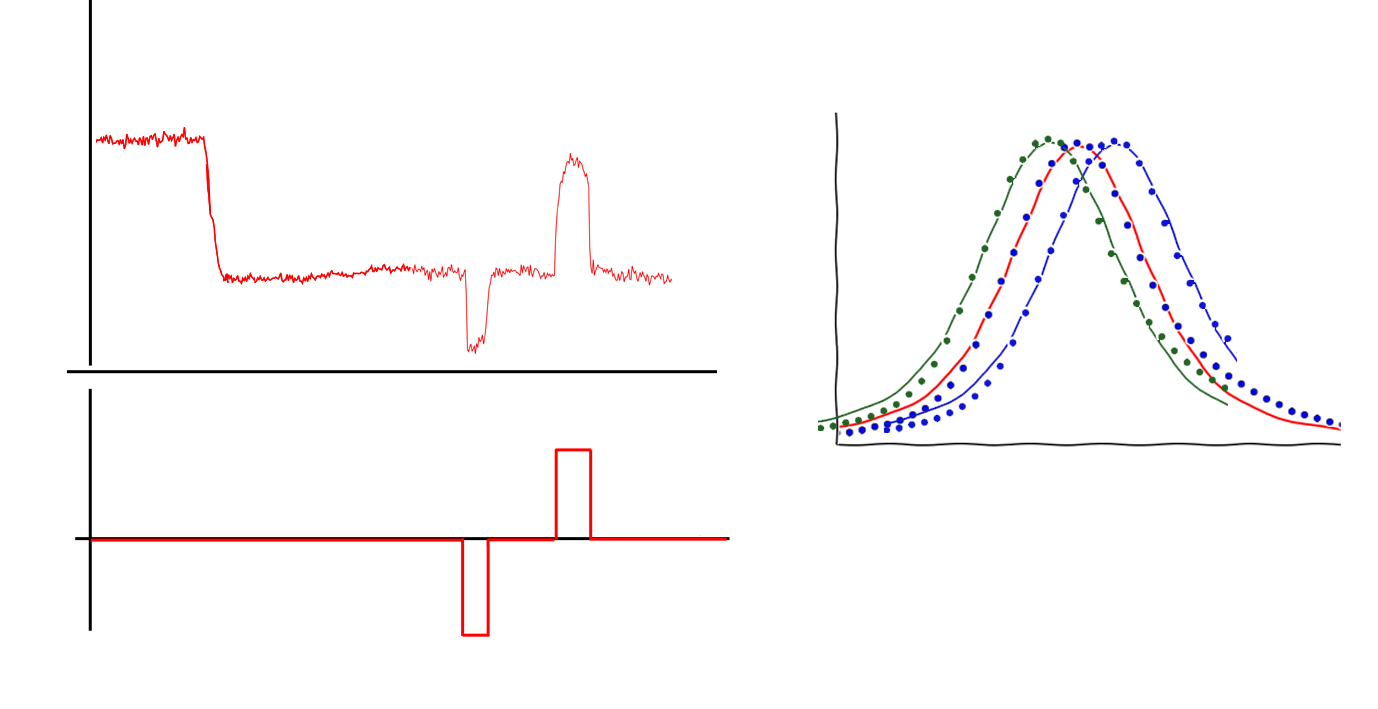
\includegraphics[width=0.8\linewidth]{images/princip.eps}
\caption{(A) Интенсивность сигнала на детекторе; (В) величина  приложенного напряжения к
поверхности кристалла; (С) восстановленное положение КДО  }
\label{ris:princip}
\end{figure}

Данный метод является наиболее быстрым, т.к. изменение интенсивности на детекторе происходит сразу,
из рисунка видно, что время за которое деформируется кристалл много меньше разрешающей способности метода.
Но дальше будет показано, что наряду с пьезоэлектрическим эффектом могут присутствовать и сопровождающие
процессы, которые ведут к не мгновенному смещению, а протекают за конечное время.

  Горфман \cite{piezo51} усовершенствовал данную методику, добавив схему совпадения, которая позволяет
  снимать двухкристальную кривую классическим методом с увеличенной временной задержкой в каждой точке отстройки.
  Увеличение времени необходимо для измерения интенсивность до момента подачи поля и после включения
   электрического поля, включение которого согласуется с помощью высокочастотного анализатора с детектором.
